\documentclass[11pt,a4paper]{article}
\usepackage{fontspec}
\setmainfont[Path=/mnt/c/Windows/Fonts/,BoldFont=timesbd.ttf,ItalicFont=timesi.ttf,BoldItalicFont=timesbi.ttf]{times.ttf}
\setmonofont[Path=/mnt/c/Windows/Fonts/,BoldFont=consolab.ttf,Scale=0.88]{consola.ttf}
\usepackage[margin=2.2cm]{geometry}
\usepackage{graphicx,float,booktabs,tabularx,array,enumitem,fancyvrb,url,caption}
\usepackage{xcolor}
\usepackage{tikz}
\usetikzlibrary{arrows.meta,positioning,fit}
\usepackage[colorlinks=true,linkcolor=blue!50!black,urlcolor=blue!50!black]{hyperref}
\linespread{1.15}
\setlength{\parskip}{4pt}
\setlist{itemsep=2pt,topsep=3pt}
\captionsetup{font=small}
\setcounter{tocdepth}{1}
\setlength{\emergencystretch}{3em}
\newcommand{\code}[1]{\texttt{\detokenize{#1}}}
\fvset{fontsize=\small,frame=single,framesep=6pt,rulecolor=\color{black!30}}
\newcolumntype{Y}{>{\raggedright\arraybackslash}X}

\title{\textbf{Camera-Based Human Motion Imitation:\\Robotis MINI in Simulation and on the Real Robot}\\[4pt]\large Final Project Midterm Report}
\author{Xiang Li}
\date{October 31, 2026}

\begin{document}
\maketitle
\thispagestyle{empty}

\begin{abstract}
\noindent
This project uses an ordinary camera and MediaPipe pose estimation to map a person's arm and leg motion, in real time, onto the 16 joints of a Robotis MINI humanoid. It was first built in MuJoCo simulation and then moved to a real MINI fitted with the KIMLAB upgrade kit. The system covers camera access under WSL2 (including streaming from Windows), limb-direction-based joint retargeting, start-up protection and smoothing, a static center-of-mass (CoM) safety filter, and a real-robot bridge that drives the XL-320 servos through a U2D2. In simulation, end-to-end latency dropped from ``several seconds and growing'' to about 0.25~s. With the CoM safety filter, all six test motions (knee lifts, a step, squats, and a sideways leg raise) stay upright in physics simulation, whereas five of them fall without it. On the real robot, communication, joint direction and zero-point calibration are done, and one 77~s full-body live imitation run was completed. Battery voltage is currently the main limit on long real-robot runs.
\end{abstract}

\tableofcontents
\vspace{1em}

%=====================================================================
\section{Overview}

\subsection{Goal}
The robot imitates the person in front of the camera in real time: when the person raises an arm, the robot raises its arm; when the person lifts a knee, the robot lifts its knee without falling over. Sides map left to left: the person's left arm drives the robot's left arm.

\subsection{System architecture}
The system is a pipeline from the camera to the joints (Figure~\ref{fig:pipeline}). Simulation and the real robot share every stage except the last one: in simulation the commands go to the MuJoCo simulator, on the real robot they go to a bridge node that forwards them to the servos through the U2D2. Both subscribe to the same ROS topic, so the imitation node itself is unchanged.

\begin{figure}[H]
\centering
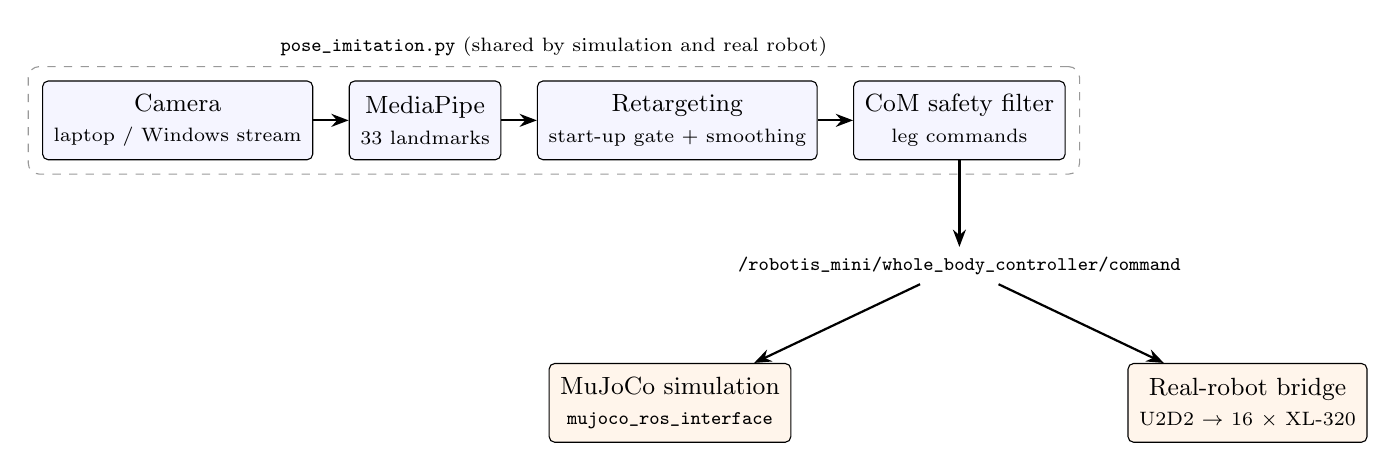
\begin{tikzpicture}[
  node distance=5mm and 4.5mm,
  box/.style={draw, rounded corners=2pt, align=center, font=\small, minimum height=10mm, inner sep=4pt, fill=blue!4},
  outbox/.style={box, fill=orange!8},
  arr/.style={-{Stealth[length=2.2mm]}, thick}]
\node[box] (cam) {Camera\\\scriptsize laptop / Windows stream};
\node[box, right=of cam] (mp) {MediaPipe\\\scriptsize 33 landmarks};
\node[box, right=of mp] (rt) {Retargeting\\\scriptsize start-up gate + smoothing};
\node[box, right=of rt] (bf) {CoM safety filter\\\scriptsize leg commands};
\node[font=\scriptsize, align=center, below=11mm of bf] (topic) {\code{/robotis_mini/whole_body_controller/command}};
\node[outbox, below left=10mm and -8mm of topic] (sim) {MuJoCo simulation\\\scriptsize \code{mujoco_ros_interface}};
\node[outbox, below right=10mm and -8mm of topic] (real) {Real-robot bridge\\\scriptsize U2D2 $\rightarrow$ 16 $\times$ XL-320};
\draw[arr] (cam) -- (mp); \draw[arr] (mp) -- (rt); \draw[arr] (rt) -- (bf);
\draw[arr] (bf) -- (topic);
\draw[arr] (topic) -- (sim); \draw[arr] (topic) -- (real);
\node[draw=black!40, dashed, rounded corners, fit=(cam)(mp)(rt)(bf), inner sep=5pt, label={[font=\scriptsize]above:\code{pose_imitation.py} (shared by simulation and real robot)}] {};
\end{tikzpicture}
\caption{System pipeline. The dashed box is the imitation node, identical for simulation and the real robot.}
\label{fig:pipeline}
\end{figure}

\subsection{Environment}
\begin{itemize}
  \item Windows laptop + WSL2 (Ubuntu 20.04), ROS Noetic, Python 3.8.
  \item MediaPipe 0.10.11 (the last release usable on Python 3.8; its jaxlib dependency no longer has a 3.8 build on PyPI, so it was installed with \code{--no-deps} and the needed dependencies were added by hand), OpenCV (opencv-contrib-python 4.10).
  \item MuJoCo 3.1.4 lives in the simulator package's own virtual environment (\path{robotis_mini_mujoco/.venv}).
  \item USB devices (cameras, U2D2) are passed into WSL with usbipd-win on Windows.
\end{itemize}

%=====================================================================
\section{Code structure}
All final-project code is in a separate ROS package, \path{~/ws_mini/src/final_project}. No assignment-2 file was modified; the simulator and robot model are reused read-only from the assignment-2 repository.

\begin{table}[H]
\centering\small
\begin{tabularx}{\textwidth}{>{\ttfamily}p{6.1cm}Y}
\toprule
\normalfont File & Purpose \\
\midrule
src/pose\_imitation.py & Imitation node: camera, MediaPipe, retargeting, CoM filter, joint command publishing; optional per-frame logging \\
src/pose\_retarget.py & Retargeting (pure numpy, testable offline): landmarks $\rightarrow$ 16 joint angles, with start-up gate and smoothing \\
src/balance\_filter.py & Static CoM safety filter: weight shift, swing-foot hold, squat-depth cap \\
src/windows\_stream.py & Receives JPEG frames streamed from Windows, keeping only the newest frame \\
src/real\_robot\_bridge.py & Real-robot bridge: joint commands $\rightarrow$ XL-320 servos, joint-state feedback, voltage/temperature protection \\
config/mujoco\_sim.yaml & Copy of the simulator config (only the unused robot head-camera rendering is disabled) \\
config/mini\_mass\_model.json & Link masses, CoM offsets and sole outlines exported from the MuJoCo model \\
config/real\_robot\_calibration.yaml & Real-robot joint map: servo ID, direction, zero point \\
launch/mujoco\_imitation.launch & Simulation + imitation \\
launch/real\_imitation.launch & Real-robot bridge + imitation \\
tools/ & Screen recording, data extraction and analysis, simulation regression test, servo scan and calibration (Section~\ref{sec:tools}) \\
\bottomrule
\end{tabularx}
\caption{Main files of the \code{final_project} package}
\end{table}

\noindent In addition, \path{~/ws_mini/vision/} contains \code{human_pose.py}, the original standalone skeleton-tracking script, and \code{win_camera_sender.py}, the Windows-side camera streamer.

%=====================================================================
\section{Camera access}

\subsection{Built-in laptop camera}
WSL2 does not see USB cameras by default. The camera is attached to WSL with usbipd on Windows:
\begin{Verbatim}
usbipd bind --busid 1-3 --force     # admin PowerShell, once
usbipd attach --wsl --busid 1-3     # after every reboot / WSL restart
\end{Verbatim}
The camera then appears as \code{/dev/video0}. Bandwidth over usbip is limited and uncompressed YUYV frames time out, so the code requests MJPG at 640$\times$480. The user must also be in the \code{video} group to read the camera.

\subsection{External USB camera (streamed from Windows)}
The external USB 2.0 PC Cam only supports uncompressed YUYV. Over usbip it loses most of its packets (the kernel log fills with \code{urb->status -104}): only the top dozen rows of each frame arrive and the rest is solid green. Lower resolutions, attaching it alone, and uvcvideo quirks did not help. The working solution bypasses usbip: Windows captures the frames with OpenCV, encodes them as JPEG and pushes them to WSL over TCP (port 5600).
\begin{Verbatim}
python.exe "$(wslpath -w ~/ws_mini/vision/win_camera_sender.py)" \
    0 $(hostname -I | cut -d' ' -f1)
\end{Verbatim}
Two details matter:
\begin{itemize}
  \item \textbf{Connect to the WSL IP, not 127.0.0.1.} 127.0.0.1 relies on Windows' wslrelay forwarding, which was seen accepting the connection without forwarding it: the sender reported ``connected'' while WSL never received a frame.
  \item \textbf{The receiver processes only the newest frame.} When the camera delivers frames faster than pose detection can process them, handling them in order lets stale frames pile up in the network buffer. Draining the buffer and keeping only the last frame on every read keeps the frame age at 0.01--0.04~s (Section~\ref{sec:latency}).
\end{itemize}

%=====================================================================
\section{Pose estimation and retargeting}

\subsection{Pose estimation}
MediaPipe Pose Landmarker (\code{pose_landmarker_full.task}, VIDEO mode, one person) outputs 33 landmarks per frame with image coordinates, 3D world coordinates and visibility. Retargeting uses only the 12 body joints (shoulders, elbows, wrists, hips, knees, ankles); fingers, toes and face points are ignored.

\subsection{Retargeting method}
\begin{enumerate}
  \item \textbf{Human torso frame}: the person's forward/left/up axes are computed from the shoulders and hips, and each limb segment (upper arm, forearm, thigh, shank) is expressed in that frame. Turning or leaning the whole body therefore does not change the arm motion relative to the body.
  \item \textbf{Per-limb joint angles}: the robot frame is x forward, y left, z up. Each arm has 3 joints (shoulder, biceps, elbow); for each leg the first 3 joints are used (hip roll, thigh, knee). A bounded least-squares fit finds the joint angles whose limb directions best match the person's. The previous frame's solution is the initial guess, with extra seeds when the fit is poor, to avoid getting stuck on the wrong branch. About 7.5~ms per frame.
  \item \textbf{Flat soles}: ankle = thigh + knee and foot roll = hip roll keep the soles parallel to the torso, which helps the robot stand.
  \item \textbf{Verification}: the hand-written kinematics match the MuJoCo model to $10^{-15}$ over 200 random joint configurations; on 10 reference poses the retargeting error is 0° for all but one.
\end{enumerate}

\paragraph{Robot limitation} After the shoulder joint rotates, the MINI's upper arm and forearm move in a single plane that always contains the robot's left--right axis. Poses such as ``upper arm hanging down, forearm pointing forward'' cannot be reproduced; the solver returns the closest pose (about 26°/64° error in the test).

\subsection{Start-up gate and smoothing}
\begin{itemize}
  \item \textbf{Start-up gate}: after start the robot holds its default stance until the whole body (shoulders, hips, knees, ankles) is inside the image and the person is standing (thighs near vertical) for about 1~s, then blends from the stance into the imitation over about 1~s. Leg landmarks must be inside the image, not only above the visibility threshold, because MediaPipe gives plausible-looking guesses for legs that are out of view.
  \item \textbf{Smoothing}: exponential smoothing of the joint commands (weight 0.3) with at most 0.4~rad change per frame. Limbs that cannot be seen hold their last pose.
\end{itemize}

%=====================================================================
\section{Center-of-mass safety filter}
\label{sec:balance}

\subsection{Why it is needed}
In early tests every leg motion that lifted a foot made the robot fall, for two reasons:
\begin{itemize}
  \item \textbf{The CoM is not moved over the stance foot}: a person shifts weight onto the other foot before lifting a leg; the robot only copied the leg angles and fell as soon as the foot left the ground.
  \item \textbf{Knee torque is insufficient}: the robot keeps its torso upright, so in a deep squat the knee sits far in front of the hip. Standing up then needs more knee torque than the XL-320's 0.39~Nm, the knee cannot straighten, and the robot falls backward.
\end{itemize}

\subsection{Method}
The filter runs after retargeting and before publishing, and only changes leg joints:
\begin{enumerate}
  \item \textbf{CoM computation}: using mass parameters exported from the MuJoCo model (\path{mini_mass_model.json}), it computes the whole-body CoM and both sole outlines (84~mm $\times$ 48~mm each) assuming an upright torso and flat soles. It matches MuJoCo exactly and takes about 0.2~ms.
  \item \textbf{Support detection}: a foot height difference below 10~mm is treated as pose-estimation jitter and the higher foot is put back on the ground (double support). Above 10~mm the filter enters single support, and returns to double support only below 5~mm (hysteresis, so jitter cannot toggle the mode).
  \item \textbf{Shift weight first, then lift}: in single support both legs roll and pitch together (soles stay flat) to move the CoM just inside the stance sole's edge (8~mm margin). Moving it only to the edge rather than the center cuts the roll from about 26° to about 15°, which the hip servos can hold. Until the CoM has arrived, the lifted leg is kept on the ground.
  \item \textbf{Squat-depth cap}: for legs on the ground, forward thigh flexion is capped at 30° (hip and knee scaled by the same factor). Simulation showed that the robot can still stand up from 30°, but falls from 40° because of knee torque.
  \item \textbf{Fallback}: if the pose is still unsafe, the legs are blended toward the default stance until it is safe.
\end{enumerate}
This is a static check and assumes fairly slow motion; fast leg lifts or kicks can still make the robot fall.

\subsection{Simulation tests}
Method: synthetic human landmarks generate slow motions (2~s to reach, 3~s hold, 2~s back). After retargeting (and the filter) they are executed at 20~Hz in MuJoCo physics simulation; the maximum torso tilt is recorded and more than 45° counts as a fall.

\begin{table}[H]
\centering\small
\begin{tabular}{lcc}
\toprule
Test motion & Without filter & With filter \\
\midrule
Left knee lift 70° & falls at 2.0 s & stands (6°) \\
Right knee lift 70° & falls at 2.0 s & stands (5°) \\
Left leg step forward 30° & falls at 3.0 s & stands (7°) \\
Right leg sideways 40° & stands (7°) & stands (12°) \\
Deep squat (thigh 80°) & falls at 6.5 s & stands (4°, squat scaled to 47\%) \\
Medium squat (thigh 40°) & falls at 6.3 s & stands (4°) \\
\midrule
Replay of a recorded run (75 s) & falls at 56.7 s (bending forward) & stands throughout (max 6°) \\
\bottomrule
\end{tabular}
\caption{Simulation tests of the CoM safety filter (maximum torso tilt in parentheses)}
\end{table}
\noindent In the replay of recorded data, standing still produced foot-height differences of up to about 5~mm from pose-estimation jitter. With the ``below 10~mm counts as jitter, put the higher foot down'' rule, the frames misclassified as single support dropped from 39\% to 0.

%=====================================================================
\section{Simulation}

\subsection{How to run}
\begin{Verbatim}
# Terminal 1: simulation + imitation (external camera streamed from Windows)
cd ~/ws_mini && source devel/setup.bash
roslaunch final_project mujoco_imitation.launch camera_source:=win
# Terminal 2: Windows-side camera streamer
cd ~/ws_mini/vision
python.exe "$(wslpath -w win_camera_sender.py)" \
    0 $(hostname -I | cut -d' ' -f1)
\end{Verbatim}
Common arguments: \code{camera_source:=0} uses the built-in laptop camera (no terminal 2 needed); \code{imitate_legs:=false} imitates the arms only; \code{balance_filter:=false} disables the CoM filter; \code{log_file:=<path>.npz} logs every frame. The top-left corner of the camera window shows the state: \code{no person}, waiting for the full body, \code{starting} (blending), \code{tracking}, plus the support state \code{[support: double/l/r]}. Backspace in the MuJoCo window resets the robot.

\subsection{Latency analysis}
\label{sec:latency}
The latency of each stage was measured separately on simulation run \code{20261031_170832}. ``Before'' values are derived from the same data; the in-order estimate assumes an unbounded queue, so in practice it is capped by the network buffer, but it still keeps growing.

\begin{table}[H]
\centering\small
\begin{tabular}{lcc}
\toprule
Stage & Before & After \\
\midrule
Network transfer (frame age) & grows; about 22 s at 60--80 s & 0.02 s \\
Smoothing & 60 ms & 20 ms \\
Pose estimation (MediaPipe etc.) & 52 ms & 52 ms \\
Robot joints following commands (in simulation) & 155 ms & 155 ms \\
\midrule
Total & seconds, still growing & about 0.25 s \\
\bottomrule
\end{tabular}
\caption{End-to-end latency (Windows-side capture, encoding and transfer not included)}
\end{table}
\noindent The largest remaining term is joint following: about 100~ms comes from the 0.1~s transition time of each command, the rest from the simulated joints' own response.

\subsection{Results}
Figure~\ref{fig:sim} shows screenshots from simulation run \code{20261031_174418} (with the CoM filter): MuJoCo on the left, the camera view on the right. This run had three single-support phases (left foot 28.1--32.1~s, right foot 36.4--40.2~s, left foot 63.4--65.1~s); each time the robot shifted its weight before lifting the leg and did not fall. Without the filter, an offline replay of the same motion falls at the first knee lift (29.9~s). At 73.4~s the robot fell once when the person rose from a deep squat in under a second, a case the filter does not yet handle (Section~\ref{sec:limits}).

\begin{figure}[H]
\centering
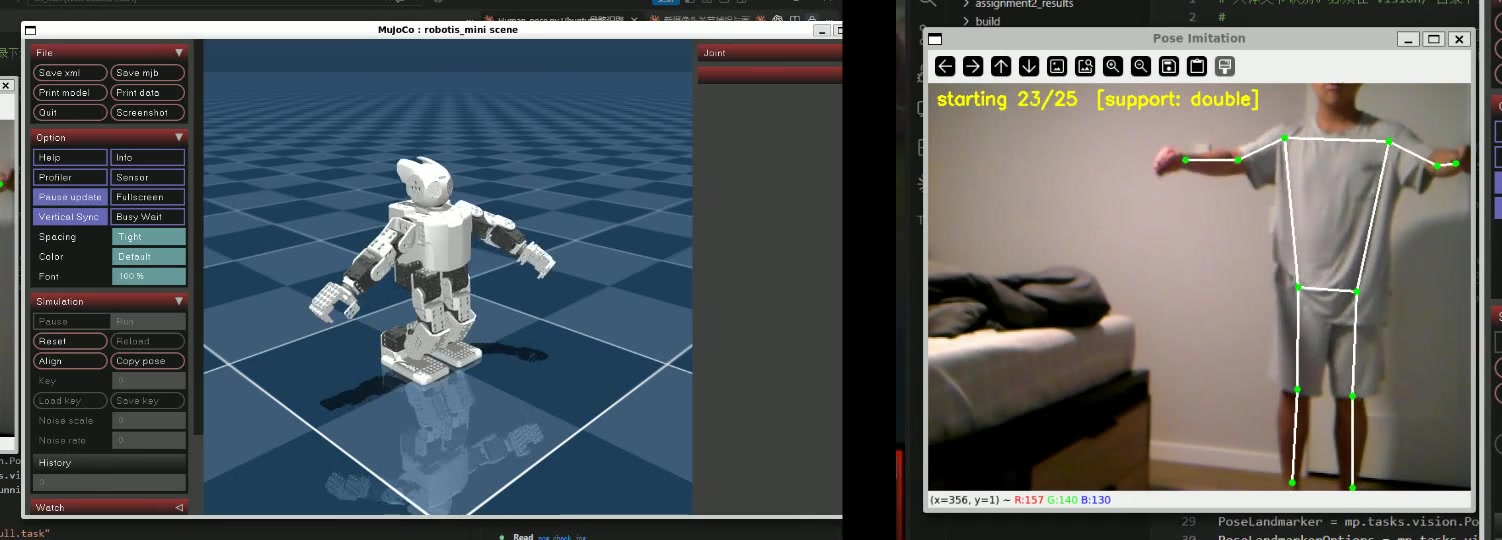
\includegraphics[width=0.49\textwidth]{figures/sim_tpose.jpg}\hfill
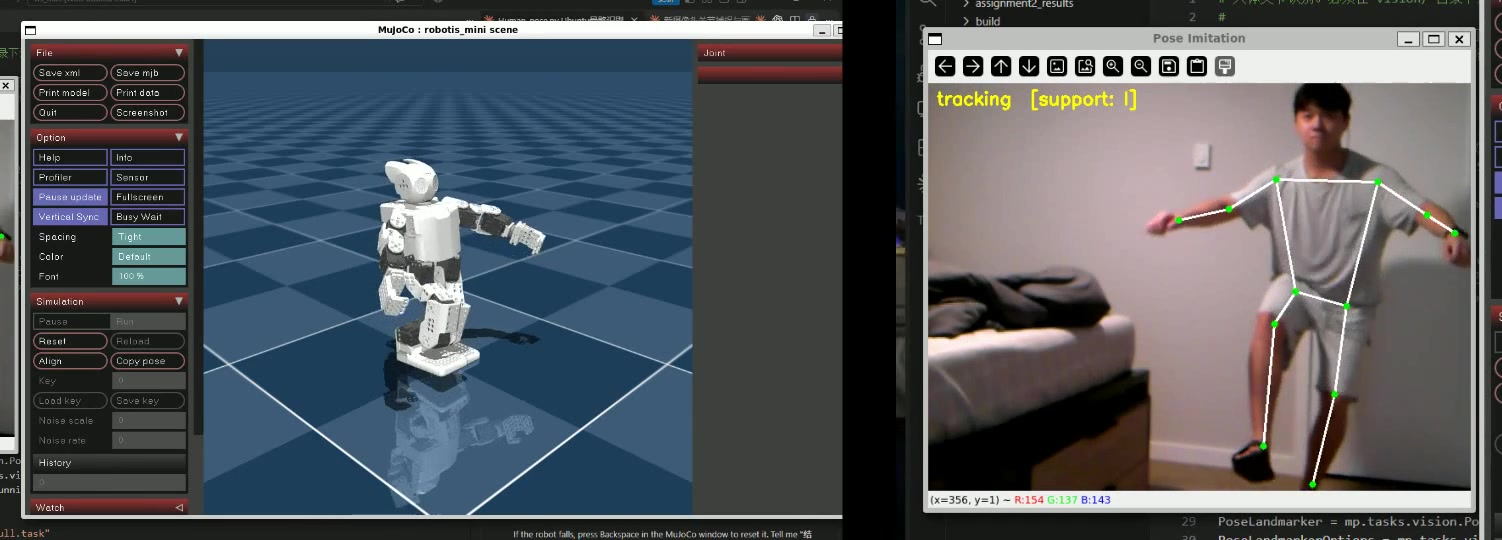
\includegraphics[width=0.49\textwidth]{figures/sim_knee_left.jpg}\\[4pt]
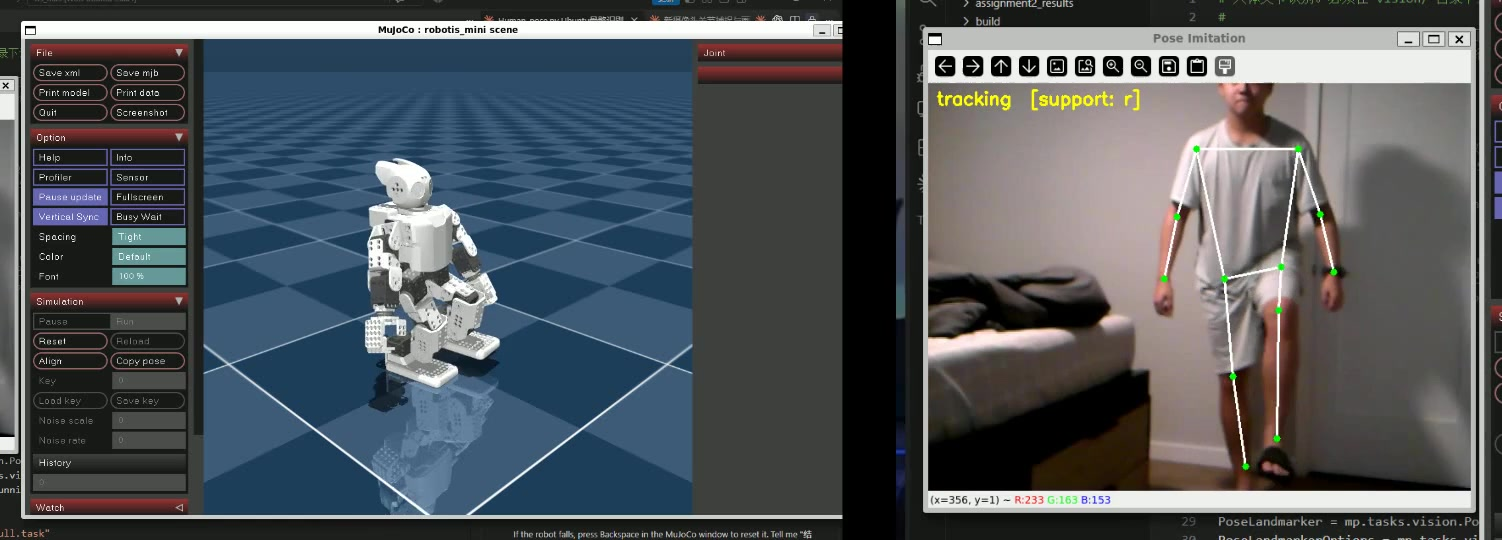
\includegraphics[width=0.49\textwidth]{figures/sim_knee_right.jpg}\hfill
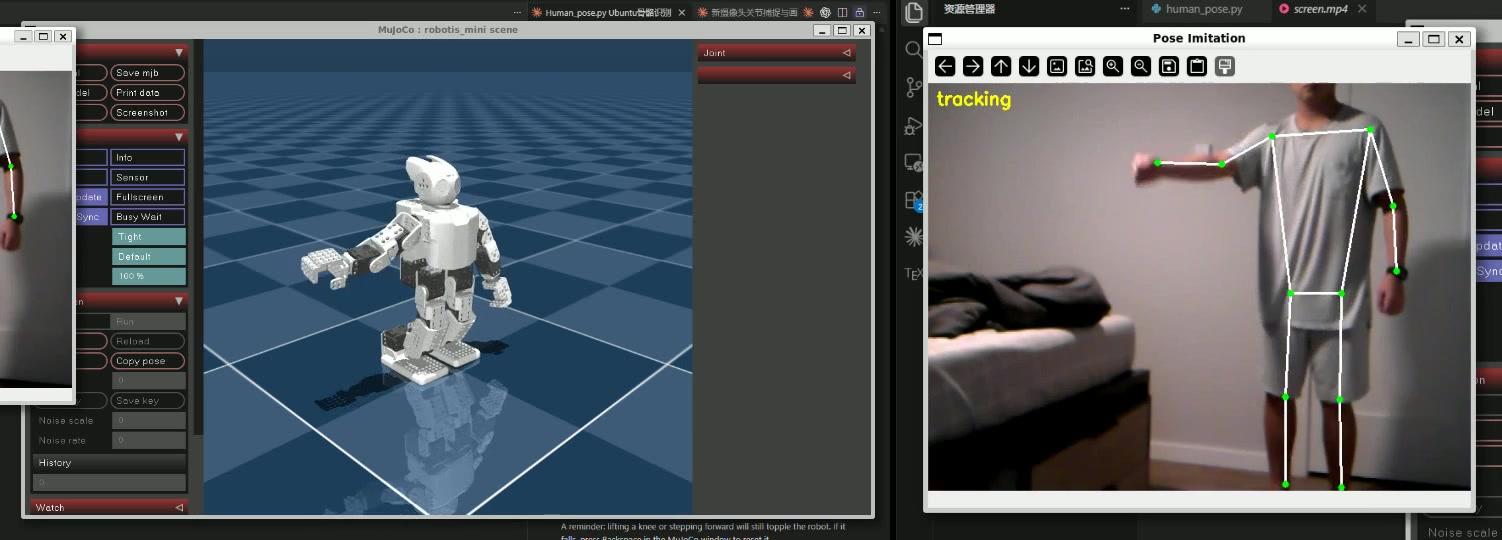
\includegraphics[width=0.49\textwidth]{figures/sim_arm_nofilter.jpg}
\caption{Simulation screenshots. Top left: start-up blending (\code{starting}), T-pose. Top right: left-foot support (\code{support: l}); the robot shifts its weight before lifting the leg. Bottom left: right-foot support (\code{support: r}). Bottom right: a run before the filter was added, one arm raised sideways.}
\label{fig:sim}
\end{figure}

%=====================================================================
\section{Real robot}

\subsection{Hardware}
The real robot is a Robotis MINI with the KIMLAB MINI upgrade kit:
\begin{itemize}
  \item 16 Dynamixel XL-320 servos (Protocol 2.0, 1~Mbps, position 0--1023, 0.293° per unit, 0.39~Nm torque limit), IDs 1--16, odd on the right and even on the left;
  \item a U2D2 USB serial adapter (FTDI chip) on the servo bus;
  \item an Orange Pi Lite 2 single-board computer, a BNO055 IMU and a USB head camera (not used at this stage);
  \item a power distribution board, powered by two 3.7~V Li-ion cells in series (about 8.4~V full) or a 7.5~V adapter.
\end{itemize}

\subsection{Connection}
In the kit the U2D2's USB goes to the Orange Pi. For debugging on the laptop, the U2D2's micro-USB cable is moved to the laptop (it must be a data cable; a charge-only cable is not recognized), then:
\begin{Verbatim}
usbipd bind --busid <BUSID> --force   # admin PowerShell, once
usbipd attach --wsl --busid <BUSID>   # after every re-plug; find BUSID with usbipd list
# lower the U2D2 latency timer from 16 ms to 1 ms:
echo 1 | sudo tee /sys/bus/usb-serial/devices/ttyUSB0/latency_timer
\end{Verbatim}
The adapter then appears as \code{/dev/ttyUSB0}; the user must be in the \code{dialout} group. The U2D2 is powered over USB, but the servos only respond when the battery or adapter is connected.

\subsection{Calibration}
\begin{enumerate}
  \item \textbf{Scan} (\code{tools/dxl_scan.py}, read-only): all 16 servos online at 1~Mbps, all XL-320, 7.4--8.0~V, 26~°C.
  \item \textbf{Directions} (\code{tools/dxl_joint_test.py}): with the robot suspended, one servo at a time is torqued and turned 10°--15° and back, and the motion is compared by eye with the motion predicted from the simulation model. Result: \textbf{IDs 1 and 2 (both shoulders) turn opposite to the simulation; the other 14 match}.
  \item \textbf{Zero points} (\code{tools/dxl_pose_test.py zero}): all 16 joints commanded to 0° reached within 2.1° of the target, and the robot matched the simulation's zero pose (arms straight out sideways, legs straight, soles flat), so no zero offsets were needed.
\end{enumerate}
The results are stored in \code{config/real_robot_calibration.yaml}: servo position $=$ 512 $+$ direction $\times$ angle (rad) $\times$ 195.38.

\subsection{Real-robot bridge}
\code{real_robot_bridge.py} subscribes to the same command topic as the simulator, so the imitation node is unchanged:
\begin{itemize}
  \item it sends all 16 goal positions with Sync Write at 50~Hz, and reads back joint angles at 10~Hz, published on \path{/robotis_mini/joint_states};
  \item \textbf{start-up}: each goal is set to the present position before torque is enabled (no jump), then the robot moves slowly to the default stance over 3~s;
  \item \textbf{limits}: every joint is clipped to the simulator's range and rate limited to 2~rad/s;
  \item \textbf{voltage and temperature protection}, checked every second: the median voltage over the 16 servos must stay below 6.3~V for 3~s in a row to stop (the bus sits 0.5--1~V below the resting voltage while the servos push, so a single reading or a brief dip must not stop the robot); any servo above 65~°C also stops it;
  \item \textbf{exit}: any exit turns all torque off. A standing robot goes limp, so hold it before stopping.
\end{itemize}

\subsection{How to run}
\begin{Verbatim}
cd ~/ws_mini && source devel/setup.bash
roslaunch final_project real_imitation.launch camera_source:=0 imitate_legs:=true
\end{Verbatim}
The real-robot launch file imitates the arms only by default (\code{imitate_legs:=false}); full-body imitation must be enabled explicitly. Keep the robot suspended on the first run; unplugging the power is the fastest emergency stop. \code{tools/replay_commands.py} replays recorded commands at their original timing without the camera (optionally arms only), to check the motion first.

\subsection{Results}
\begin{table}[H]
\centering\small
\begin{tabularx}{\textwidth}{lY}
\toprule
Run & Result \\
\midrule
\code{real_20261031_185703} & Full 77~s run, stopped by hand. Pose estimation at 18.5~fps; waiting for the full body from 4.0~s, blending at 30.3~s, tracking from 32.0~s; 647 tracking frames (about 45~s), 19 of them single support. Bus voltage 6.8--7.0~V under load, servo temperature at most 32~°C, no communication drop-outs. \\
\code{real_20261031_185928} & After about 56~s the bus voltage stayed at 6.2~V for 3~s and the bridge stopped and turned torque off as designed. The resting voltage measured afterward was 7.3~V median (about 3.65~V per cell, roughly 30--40\% charge left). \\
\bottomrule
\end{tabularx}
\caption{Real-robot runs}
\end{table}
\noindent Neither real-robot run was screen-recorded, so this document does not describe how the robot's motion actually looked (direction, range, naturalness); video should be added in later tests.

%=====================================================================
\section{Known limitations and future work}
\label{sec:limits}
\begin{itemize}
  \item \textbf{Fast standing up}: rising from a deep squat in under a second outruns the knee torque and the robot falls backward. The knee extension speed of loaded legs could be limited, and the squat cap tightened from 30° to about 25°.
  \item \textbf{Static filter}: the CoM filter only checks static stability and ignores inertia and sway during motion. A next step is to use the IMU (available in simulation; the real kit has a BNO055) to correct the ankles and hips from the actual torso tilt.
  \item \textbf{Torso lean}: the robot's torso always stays upright and does not imitate bending forward; when the person bends, the squat cap and CoM filter keep the robot safe.
  \item \textbf{Arm structure}: the MINI cannot reproduce ``upper arm down, forearm forward''.
  \item \textbf{Real-robot power}: at 30--40\% battery, servo load pulls the bus to about 6.2~V, close to the XL-320's minimum operating voltage. A 7.5~V adapter (2.5$\times$5.5~mm, at least 2~A) is recommended for long sessions.
  \item \textbf{Wireless operation}: the U2D2 is currently connected to the laptop over USB. The bridge could run on the robot's Orange Pi, with the laptop sending commands over Wi-Fi via ROS.
  \item \textbf{Pose-estimation speed}: the two kept simulation recordings ran at 13.4 and 11.0~fps, while the real-robot run (not screen-recorded) ran at 18.5~fps. Screen recording and simulation are suspected to take the CPU, but this was not verified separately.
\end{itemize}

%=====================================================================
\section{Tools}
\label{sec:tools}
\begin{table}[H]
\centering\small
\begin{tabularx}{\textwidth}{>{\ttfamily}p{4.6cm}Y}
\toprule
\normalfont Tool (\code{tools/}) & Purpose \\
\midrule
record\_windows.py & Records the MuJoCo and camera windows on Windows (pinned on top, side by side) to mp4; convert to H.264 with ffmpeg afterward \\
extract\_bag.py & Extracts the rosbag of a recording into npz \\
analyze\_run.py & Analyzes a simulation recording: latency, smoothing, joint following, standing \\
export\_mass\_model.py & Exports the mass parameters for the CoM filter from the MuJoCo model \\
test\_balance\_filter.py & Simulation regression test of the CoM filter (with synthetic\_human.py) \\
dxl\_scan.py & Scans the servos: ID, model, position, voltage, temperature (read-only) \\
dxl\_joint\_test.py & Single-joint direction test \\
dxl\_pose\_test.py & Moves the whole body to a pose (0° or the default stance) \\
joint\_test\_plan.py & Predicts, from the simulation model, how each joint test should move \\
replay\_commands.py & Replays recorded joint commands at their original timing \\
\bottomrule
\end{tabularx}
\caption{Helper tools}
\end{table}

%=====================================================================
\newpage
\section{Recorded data}
The kept recordings are packed in \code{recordings.zip} (three real-robot runs that failed at start-up without useful data were deleted):
\begin{table}[H]
\centering\small
\begin{tabularx}{\textwidth}{>{\ttfamily}p{4.4cm}Y}
\toprule
\normalfont Directory & Contents \\
\midrule
20261031\_170832 & Simulation before the CoM filter. Source of the latency analysis; includes the fall when bending forward at 56~s. 55~s screen recording (\code{screen.mp4}) \\
20261031\_174418 & Simulation with the CoM filter. Knee lifts and squats; 44~s screen recording (original 9--53~s) \\
real\_20261031\_185703 & Real robot, full 77~s run \\
real\_20261031\_185928 & Real robot, stopped automatically after 56~s on low battery voltage \\
\bottomrule
\end{tabularx}
\caption{Kept recordings}
\end{table}
\noindent In each directory, \code{frames.npz} holds per-frame data (landmarks, processing time, dropped stale frames, joint commands before and after the filter, support state). Simulation directories also contain \code{robot.bag} (joint angles, torso pose, commands), \code{robot_extracted.npz} and the screen recording \code{screen.mp4} (H.264); \code{launch.log} and the other logs are run logs. Only the videos were trimmed; the data files cover the full runs.

%=====================================================================
\section{Troubleshooting}
\begin{table}[H]
\centering\small
\begin{tabularx}{\textwidth}{p{4.8cm}Y}
\toprule
Symptom & Cause and fix \\
\midrule
No \code{/dev/video0} & Camera not attached to WSL: \code{usbipd attach --wsl --busid 1-3} \\
Frame read timeout (select timeout) & Make sure the code requests MJPG \\
External camera shows green frames & That camera cannot be used over usbip; stream it from Windows \\
Streamer says connected, no window & wslrelay is not forwarding: pass the WSL IP, not 127.0.0.1 \\
Latency keeps growing & The receiver must keep only the newest frame (current code does) \\
Laptop does not see the U2D2 & Charge-only cable, use a data cable; or the U2D2 is still on the Orange Pi \\
U2D2 present, servos do not answer & Robot not powered (servos need battery or adapter) \\
Occasional ``no status packet'' & Sporadic packet loss over USB passthrough; tools and bridge retry automatically \\
Bridge stops on low voltage & Battery low or sagging too much under load: charge it or use a 7.5~V adapter \\
\bottomrule
\end{tabularx}
\caption{Troubleshooting}
\end{table}

\end{document}
